% Dieser Text ist urheberrechtlich geschützt
% Er stellt einen Auszug eines von mir erstellten Referates dar
% und darf nicht gewerblich genutzt werden
% die private bzw. Studiums bezogen Nutzung ist frei
% Mai 2005 
% Autor: Sascha Frank 
% Universität Freiburg 
% www.informatik.uni-freiburg.de/~frank/
%
%  zusaetzlich ist das usepackage{beamerthemeshadow} eingebunden 
%  
%  \beamersetuncovermixins{\opaqueness<1>{25}}{\opaqueness<2->{15}}
%  sorgt dafuer das die Elemente die erst noch kommen nur schwach 
%  angedeutet erscheinen 
\documentclass{beamer}
\usepackage[ngerman]{babel}
\usepackage[utf8]{inputenc}
\usepackage[T1]{fontenc}
\usepackage{movie15}
\usepackage{beamerthemeshadow}
\beamersetuncovermixins{\opaqueness<1>{25}}{\opaqueness<2->{15}}
\begin{document}
\title{Visuelle Analyse zur Erfassung eines Dartspiels}  
\author{Maximilian Hertzer}
\date{\today} 

\frame{\titlepage} 

\frame{\frametitle{Ablauf}\tableofcontents} 


\section{Einleitende Worte} 
\subsection{Motivation}
\begin{frame}{Motivation} 
\begin{itemize}
\item Dartsport wird immer beliebter \pause
\item Preisgelder steigen \pause
\item Wettbewerberniveau steigt \pause
\item Training sollte überwacht werden \pause
\item Beim Steeldart gibt es keine automatisierte Möglichkeit Würfe zu erfassen
\item Spiele für Hobbyspieler ermöglichen
\end{itemize} 
\end{frame}

\subsection{Ziel der Arbeit }
\begin{frame}{Ziel der Arbeit} 
\begin{itemize}
\item Automatische Erkennung von Darts ermöglichen 
\item Die Kosten gering halten 
\item Überwachung von Trainingserfolgen
\end{itemize} 
\end{frame}


\section{Umsetzung} 
\frame{\frametitle{Umsetzung}
\begin{overprint}
\centering
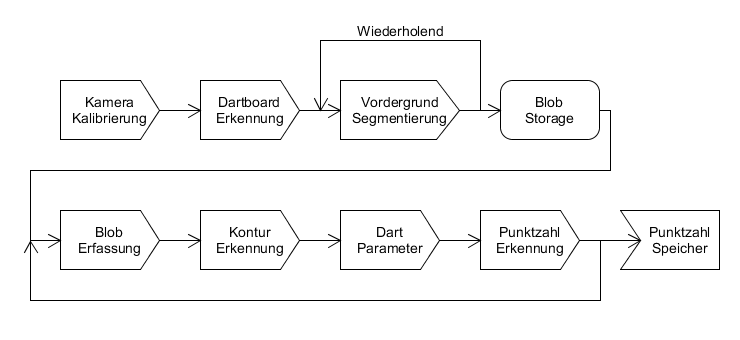
\includegraphics[scale=0.36]{./media/pipeline.png}

\end{overprint}
}
\subsection{Kalibrierung}
\frame{\frametitle{Kamerakalibrierung}
\begin{itemize}
\item Intrinsische Parameter der Kamera bestimmen \pause
\item Focal Length
\item Cetroid
\item Verzerrungsparameter 
\end{itemize} 
}

\frame{\frametitle{Kamerakalibrierung}
\begin{overprint}
\begin{figure}


\centering
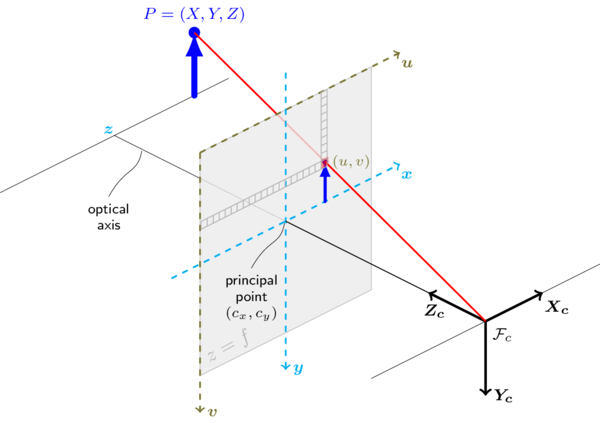
\includegraphics[scale=0.35]{./media/pinhole_camera_model.png}
\caption{Camera Calibration and 3D Reconstruction;\newline
Itseez Inc. 2016; Abgerufen: 01.02.2017 }
\end{figure}
\end{overprint}
}

\frame{\frametitle{Kamerakalibrierung}
\begin{itemize}
\item Intrinsische Parameter der Kamera bestimmen 
\item Focal Length
\item Cetroid
\item Verzerrungsparameter 
\item Verwendung von Schachbrettmuster zur Featurepunktbestimmung
\end{itemize} 
}

\frame{\frametitle{Kamerakalibrierung}
\begin{overprint}
\centering
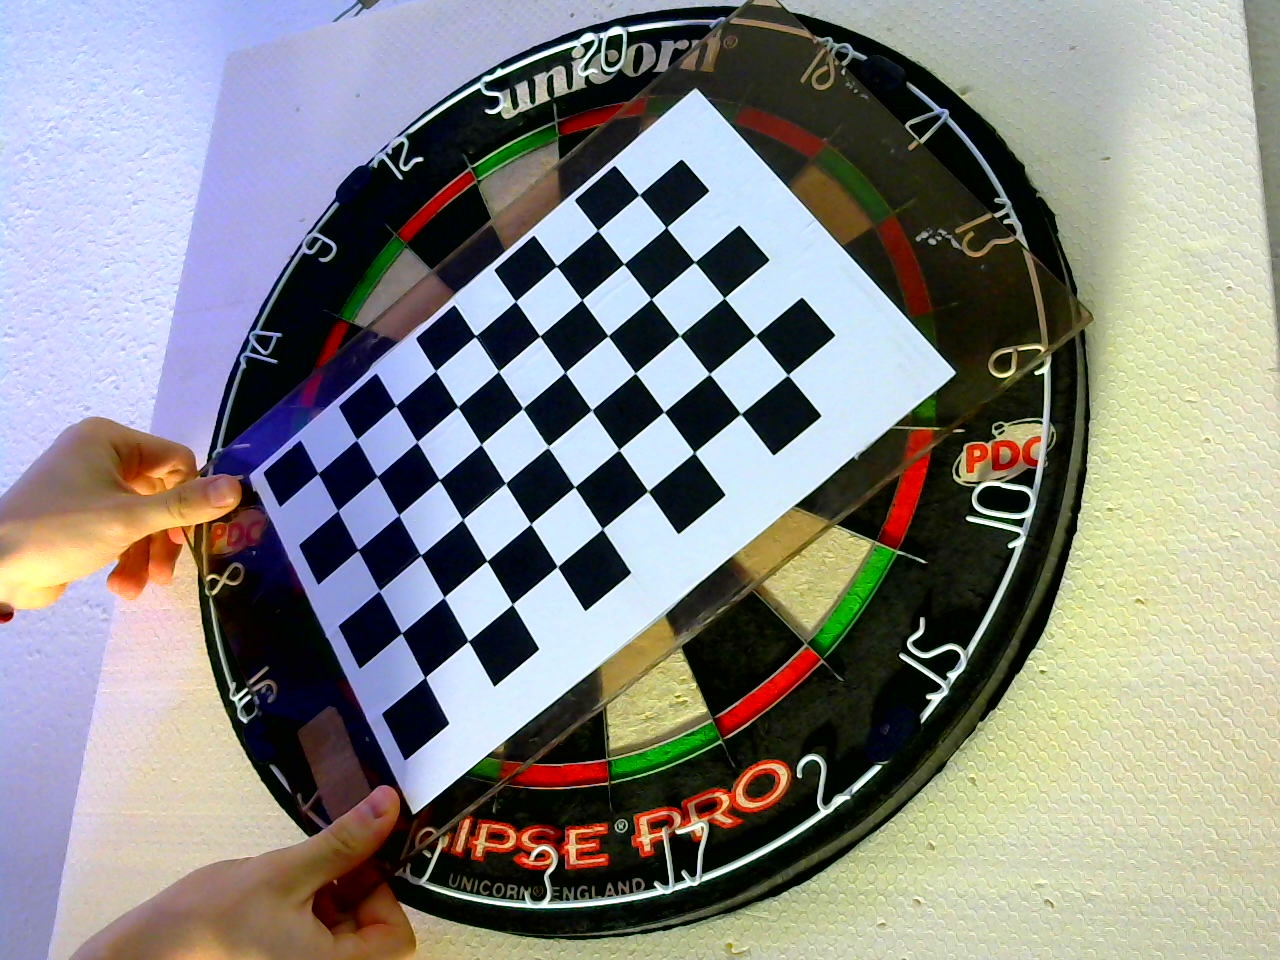
\includegraphics[scale=0.2]{./media/calibraw1.jpg}

\end{overprint}
}
\frame{\frametitle{Kamerakalibrierung}
\begin{overprint}
\centering
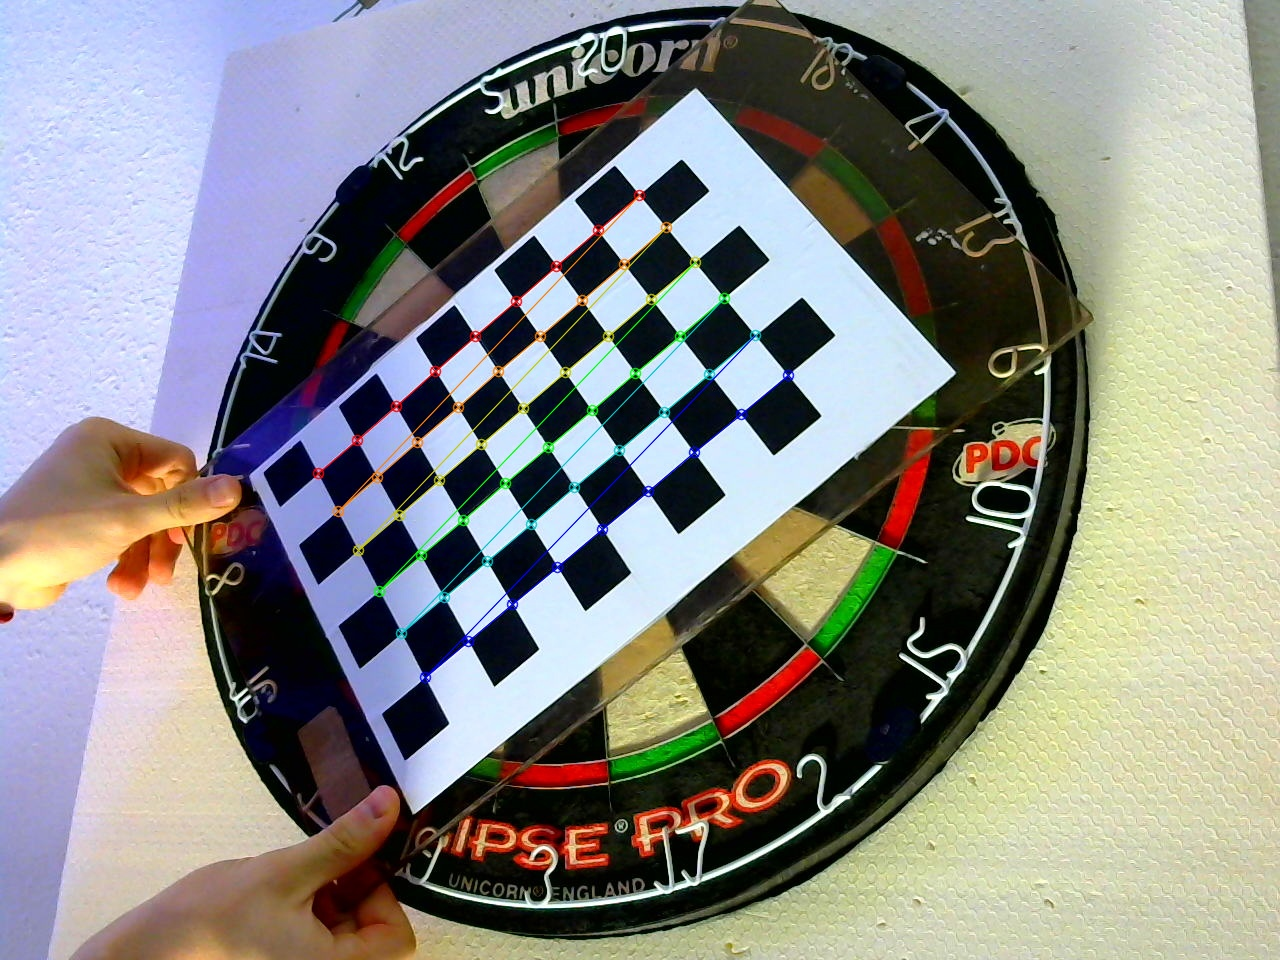
\includegraphics[scale=0.2]{./media/calibrated1.jpg}

\end{overprint}
}

\frame{\frametitle{Dartboardkalibrierung}
\begin{itemize}
\item Extrinsische Parameter bestimmen \pause
\item Rotationsmatrix
\item Translationsmatrix \pause
\item Interaktion mit dem Nutzer
\end{itemize} 
}

\frame{\frametitle{Dartboardkalibrierung}
\begin{overprint}
\centering
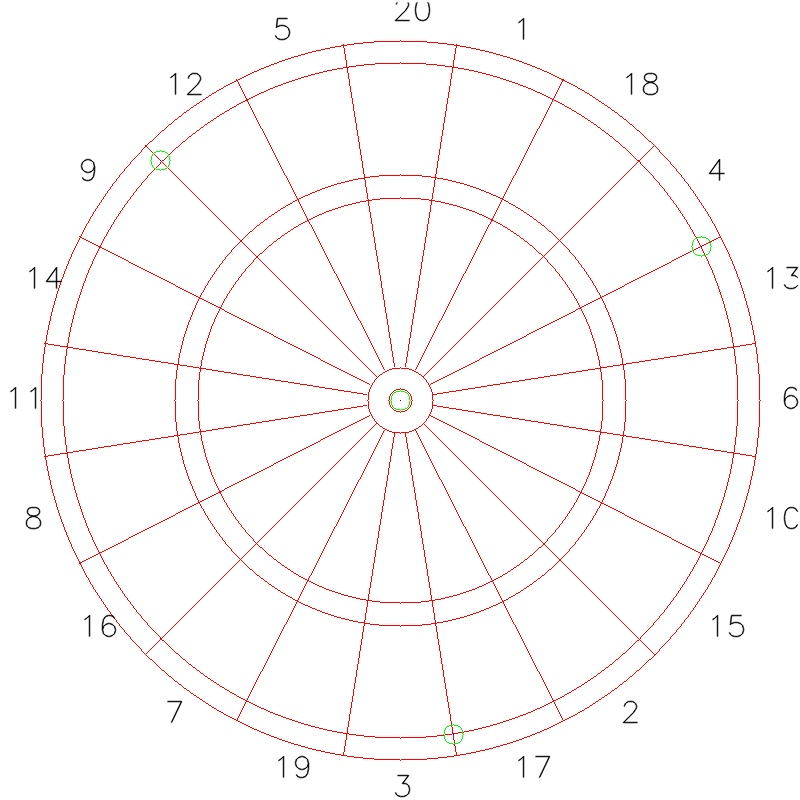
\includegraphics[scale=0.2]{./media/confighints.jpg}

\end{overprint}
}



\subsection{Darts Segmentierung}
\frame{\frametitle{Darts Segmentierung}
\begin{overprint}
\centering
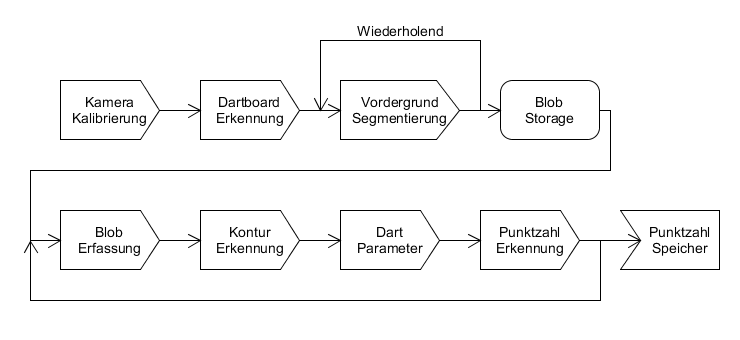
\includegraphics[scale=0.36]{./media/pipeline.png}

\end{overprint}
}
%\frame{\frametitle{Blob Erfassung}
%\begin{enumerate}
%\item  Einf\"uhrungskurs in \LaTeX \pause 
%\item  Kurs 2 \pause 
%\item  Seminararbeiten und Pr\"asentationen mit \LaTeX \pause 
%\item  Die Beamerclass
%\end{enumerate}
%}

\frame{\frametitle{Background Substraction}
\begin{enumerate}
\item  Hintergrundmodell erstellen \pause 
\item  Aktuelles Bild vom Hintergrund subtrahieren
\item  Optional Hintergrundmodell aktualisieren \pause 
\item  Thresholding anwenden \pause 
\item  Vordergrundmaske wird gebildet
\end{enumerate}
}

\frame{\frametitle{Background Substraction}
\begin{overprint}
\centering
\centerline{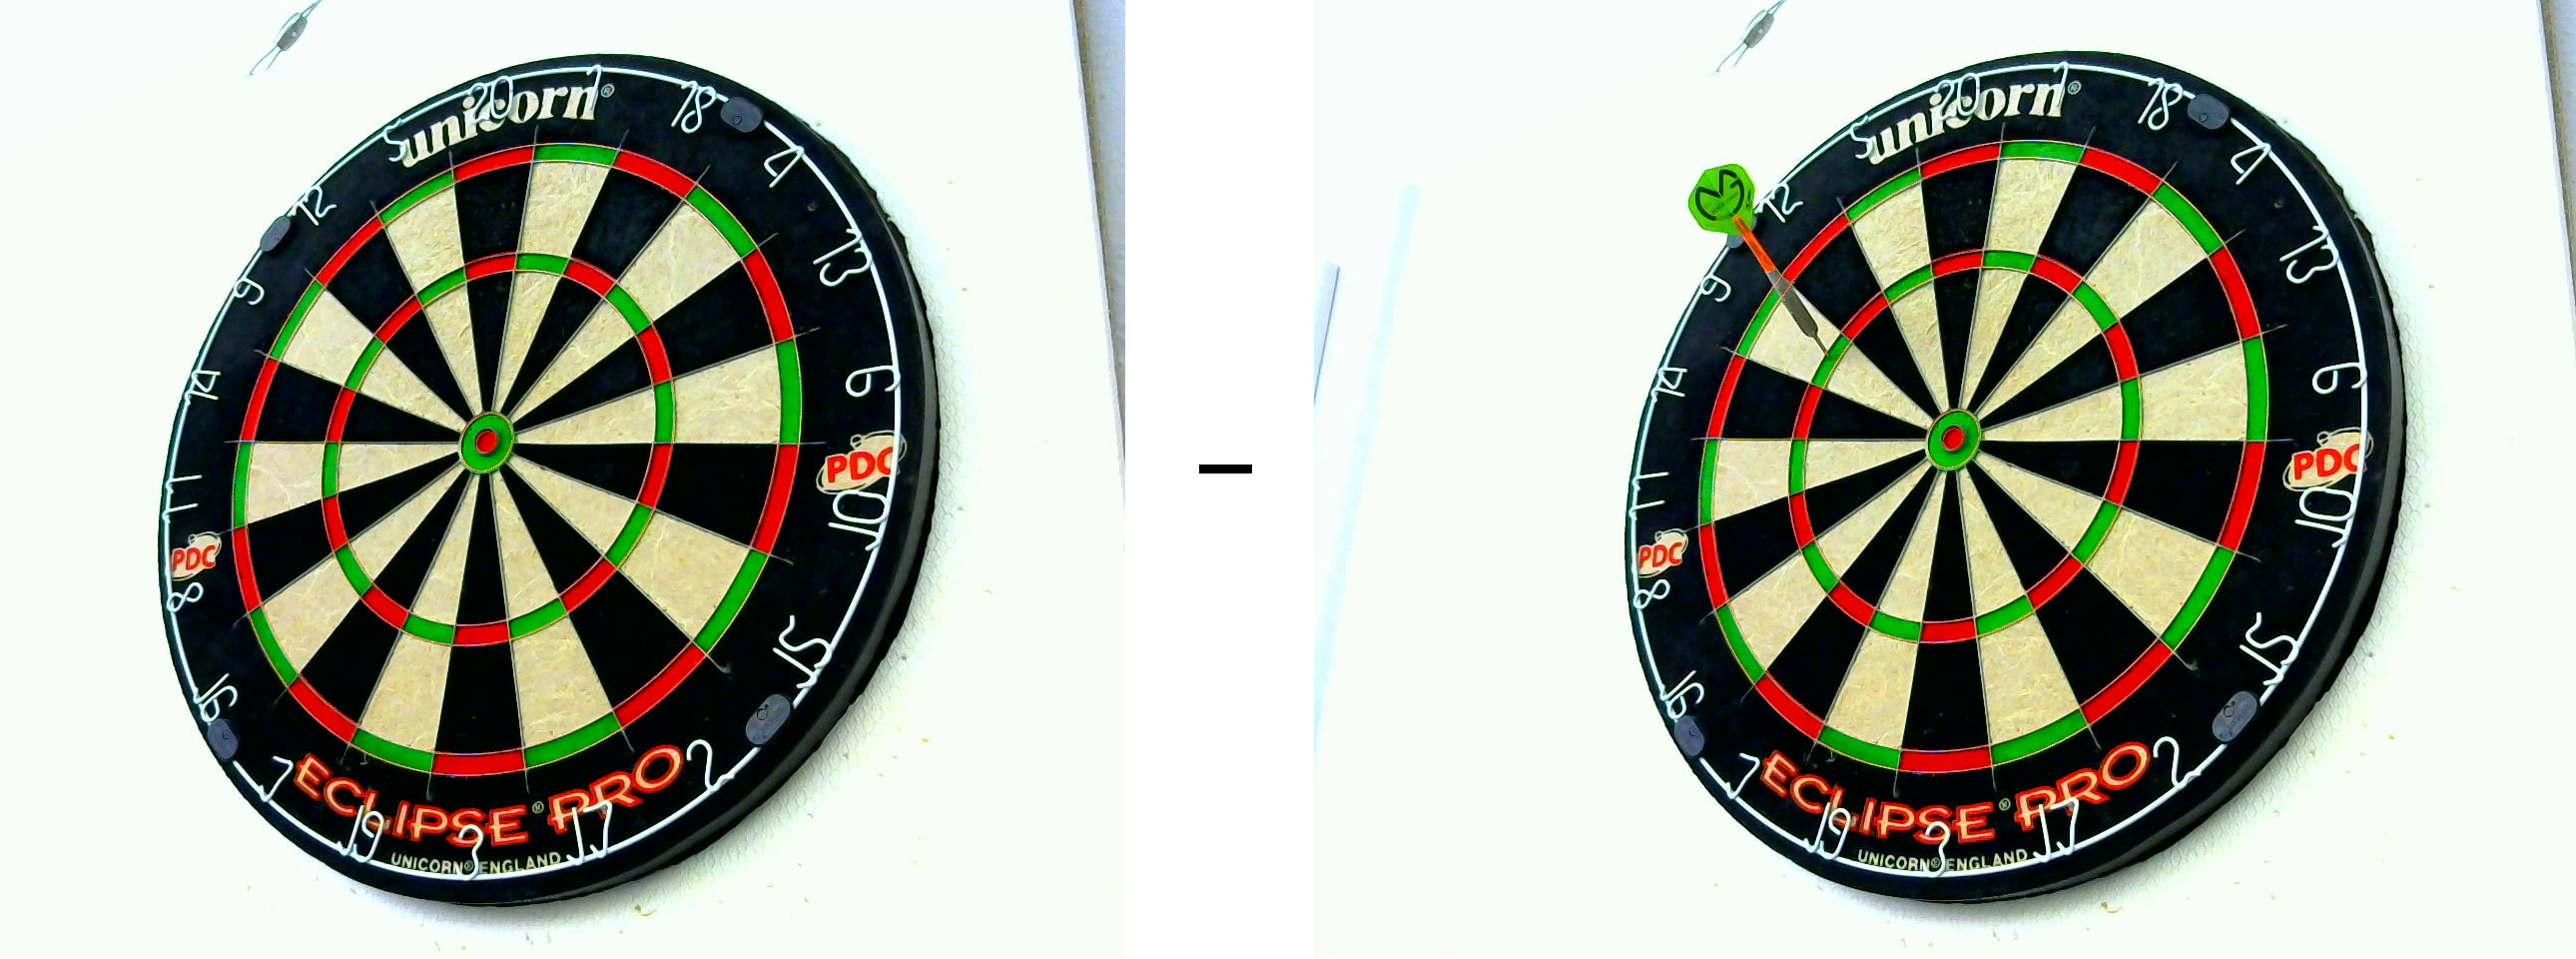
\includegraphics[scale=0.12]{./media/backgroundsub.jpg}}
%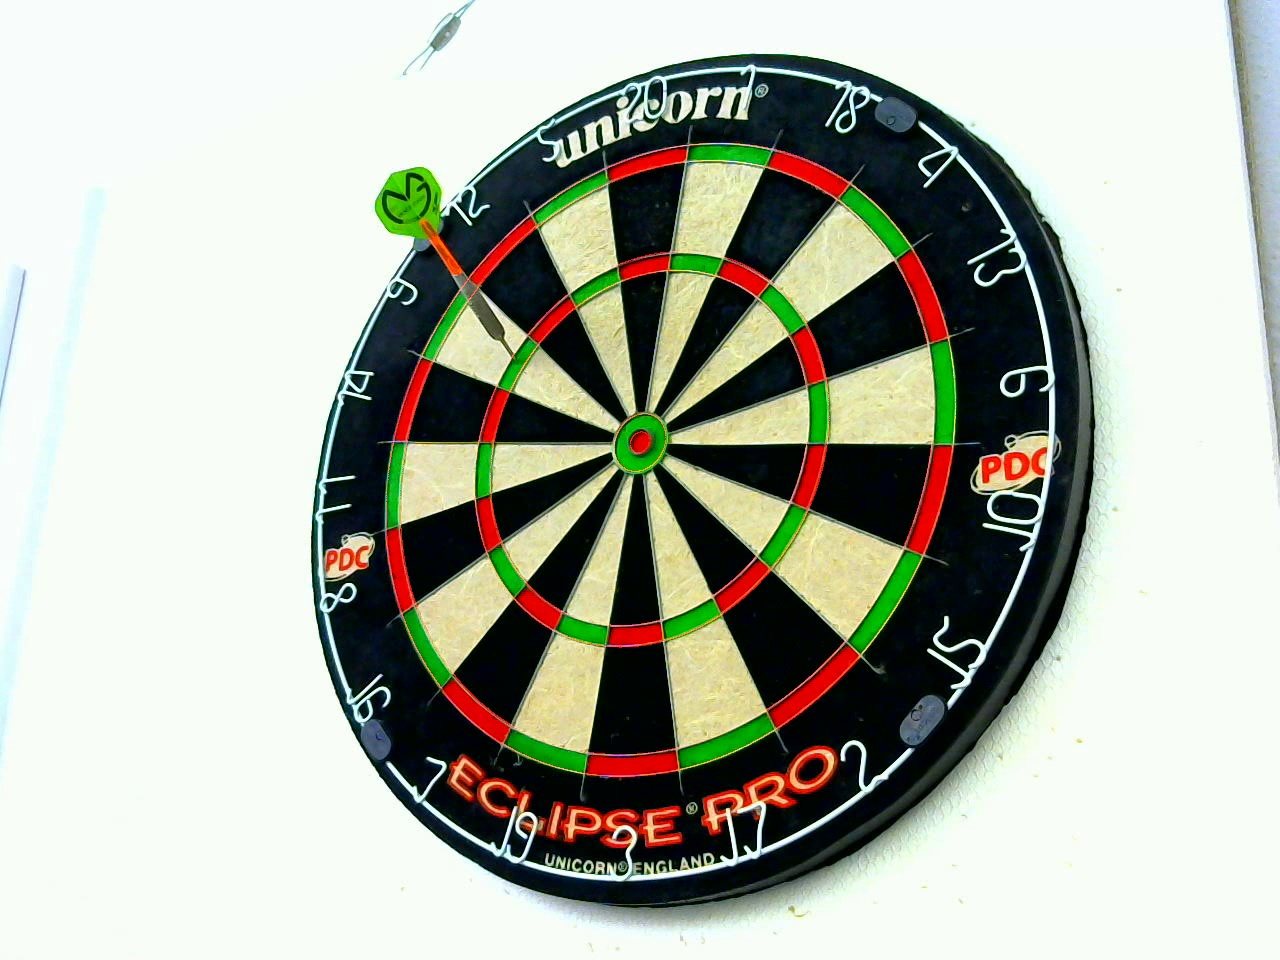
\includegraphics[scale=0.1]{./media/current.jpg}
\end{overprint}
}


\frame{\frametitle{Vordergrundmaske}
\begin{overprint}
\centering
\centerline{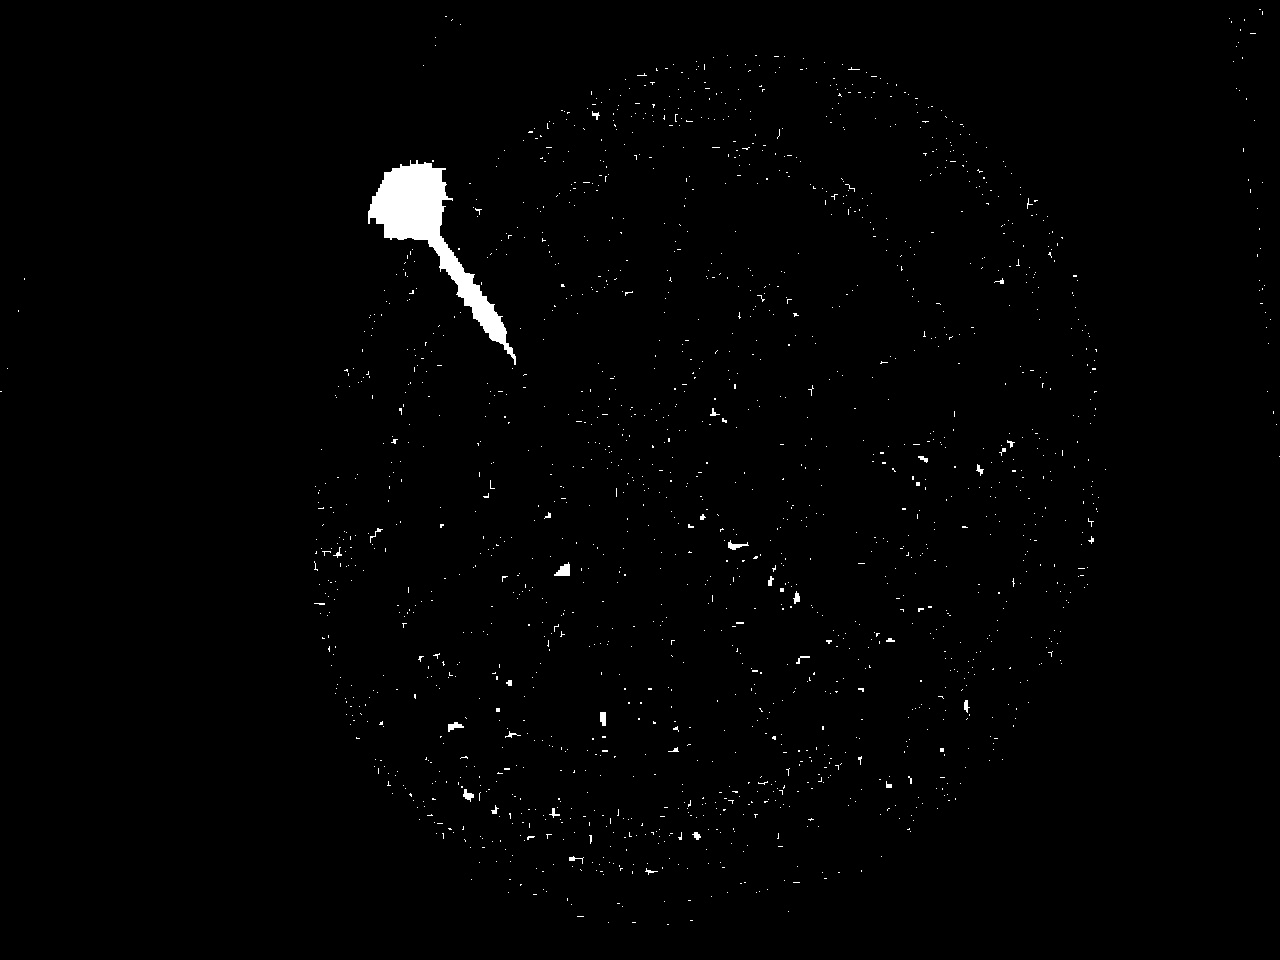
\includegraphics[scale=0.15]{./media/substracted.jpg}}
%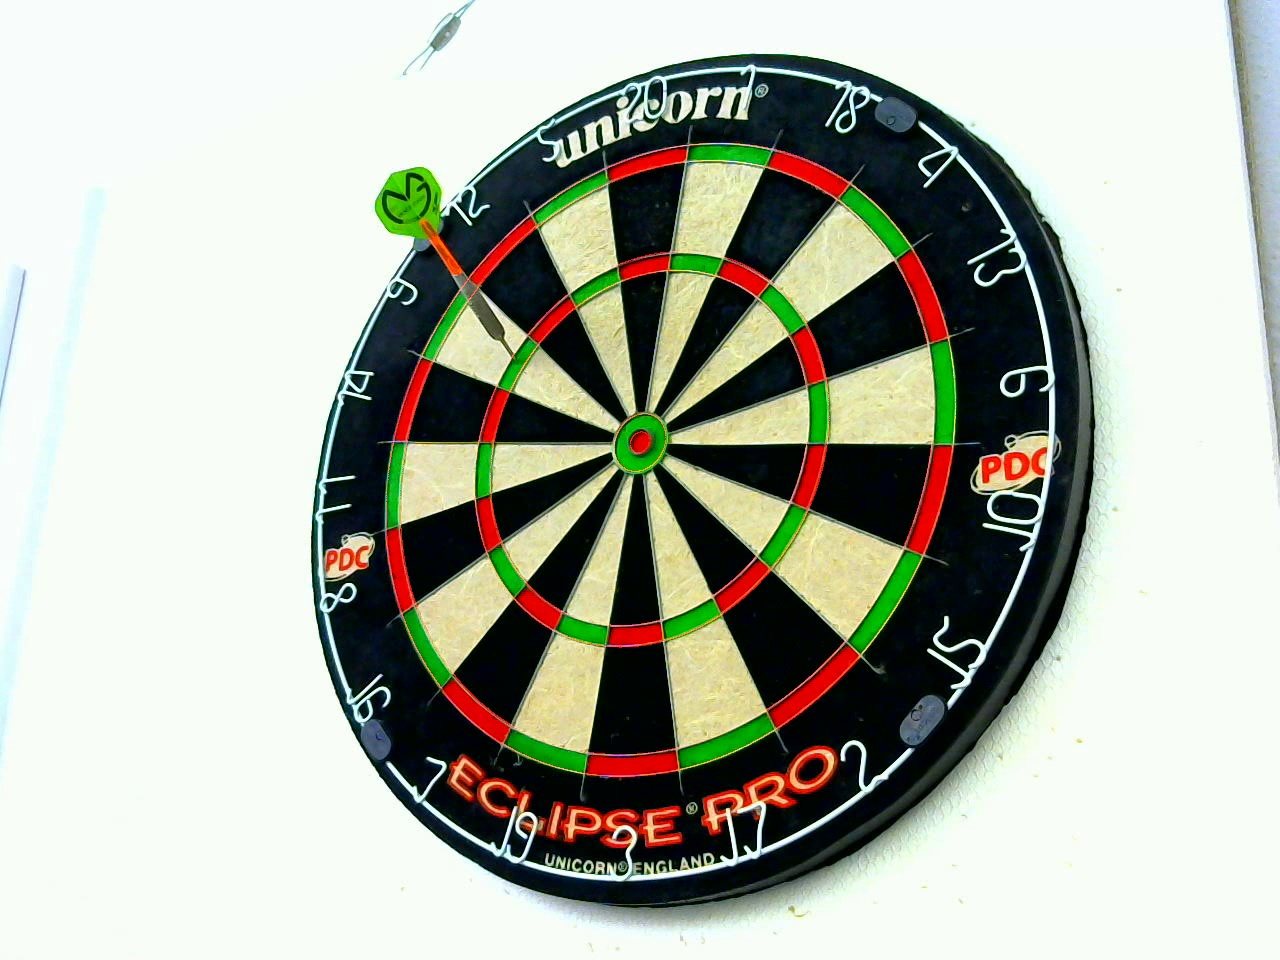
\includegraphics[scale=0.1]{./media/current.jpg}
\end{overprint}
}


\frame{\frametitle{Blob Erfassung}
\begin{enumerate}
\item  Zusammenhängende Bereiche in der Vordergrundmaske erkennen\pause 
\item  Anzahl der Pixel dieser Bereiche bestimmen\pause
\item  Bild und größten Bereich dem Storage hinzufügen 
\end{enumerate}
}

\frame{\frametitle{Blob Erfassung}
\begin{overprint}
\centering
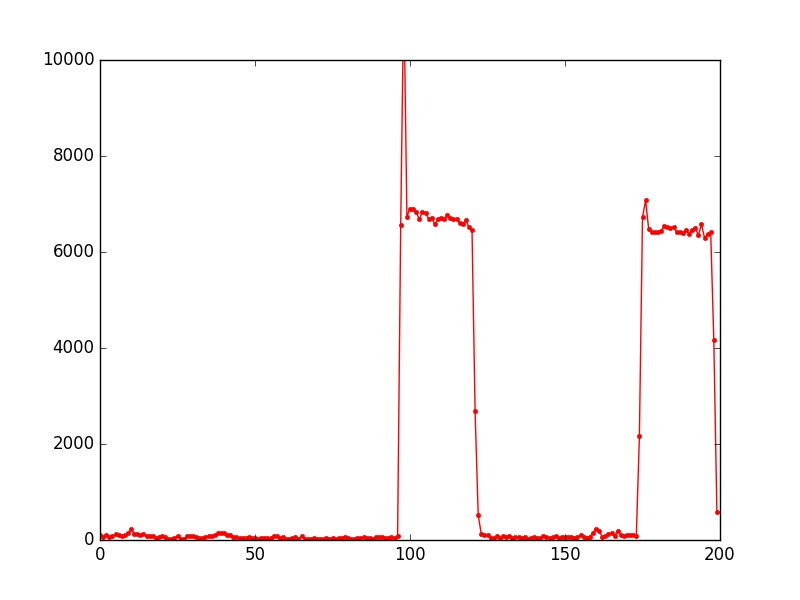
\includegraphics[scale=0.32]{./media/plot.jpg}

\end{overprint}
}

\frame{\frametitle{Blob Erfassung}
\begin{overprint}
\centering
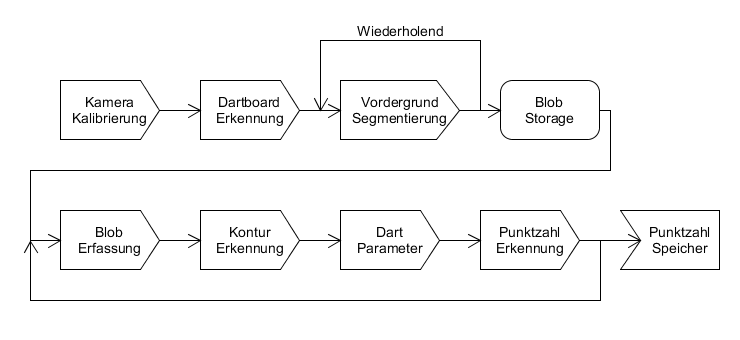
\includegraphics[scale=0.36]{./media/pipeline.png}

\end{overprint}
}

\frame{\frametitle{Blob Erfassung}
\begin{enumerate}
\item  Bereiche in denen ein Dart sichtbar ist bestimmen \pause 
\item  Bereiche mit zu großem Vordergrund ausfiltern
\end{enumerate}
}

\frame{\frametitle{Blob Erfassung}
\begin{overprint}
\centering
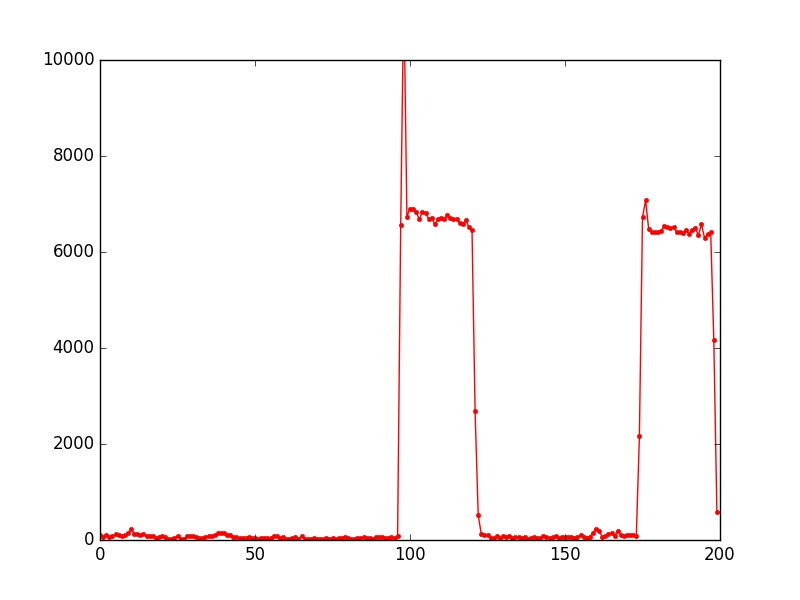
\includegraphics[scale=0.32]{./media/plot.jpg}

\end{overprint}
}

\frame{\frametitle{Blob Erfassung}
\begin{itemize}

\item  Zusammenhängender Bereich 98 bis 120 \pause 
\item  Jede Vordergrundmaske des Bereiches betrachtet \pause
\item  Leeres Graustufenbild erstellen \pause
\item  Für jeden zum Vordergrund gehörigen Pixel: Grauwert erhöhen \pause
\item Thresholding auf Graustufenbild anwenden
\end{itemize}
}

\frame{\frametitle{Blob Erfassung}
\begin{overprint}
\centering
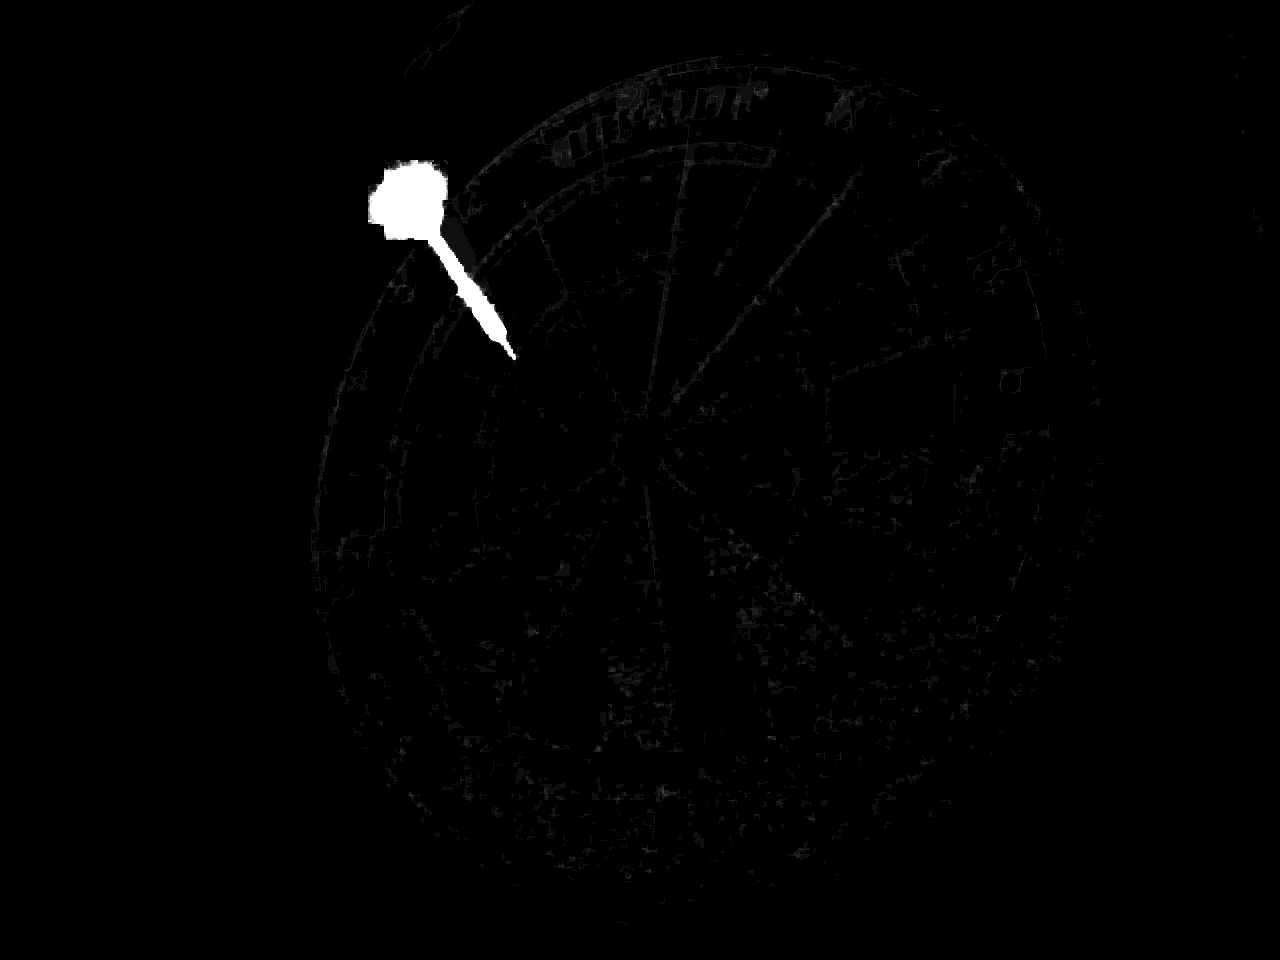
\includegraphics[scale=0.18]{./media/blobimg.jpg}

\end{overprint}
}

\frame{\frametitle{Kontur Erkennung}
\begin{overprint}
\centering
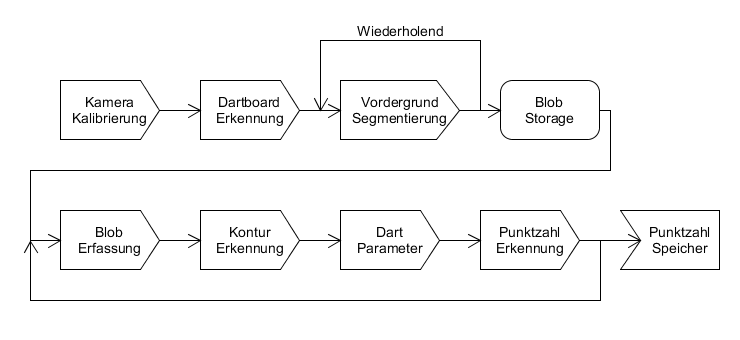
\includegraphics[scale=0.36]{./media/pipeline.png}

\end{overprint}
}

\frame{\frametitle{Kontur Erkennung}
\begin{itemize}
\item  Kontur auf dem resultierenden Binärbild erkennen \pause 
\item  Anhand der Kontur die Momente und Features bestimmen \pause
\item  Gerade durch die Kontur \pause
\item  Schwerpunkt der Kontur \pause
\item  Bounding rectangle
\end{itemize}
}

\frame{\frametitle{Kontur Erkennung}
\begin{overprint}
\centering
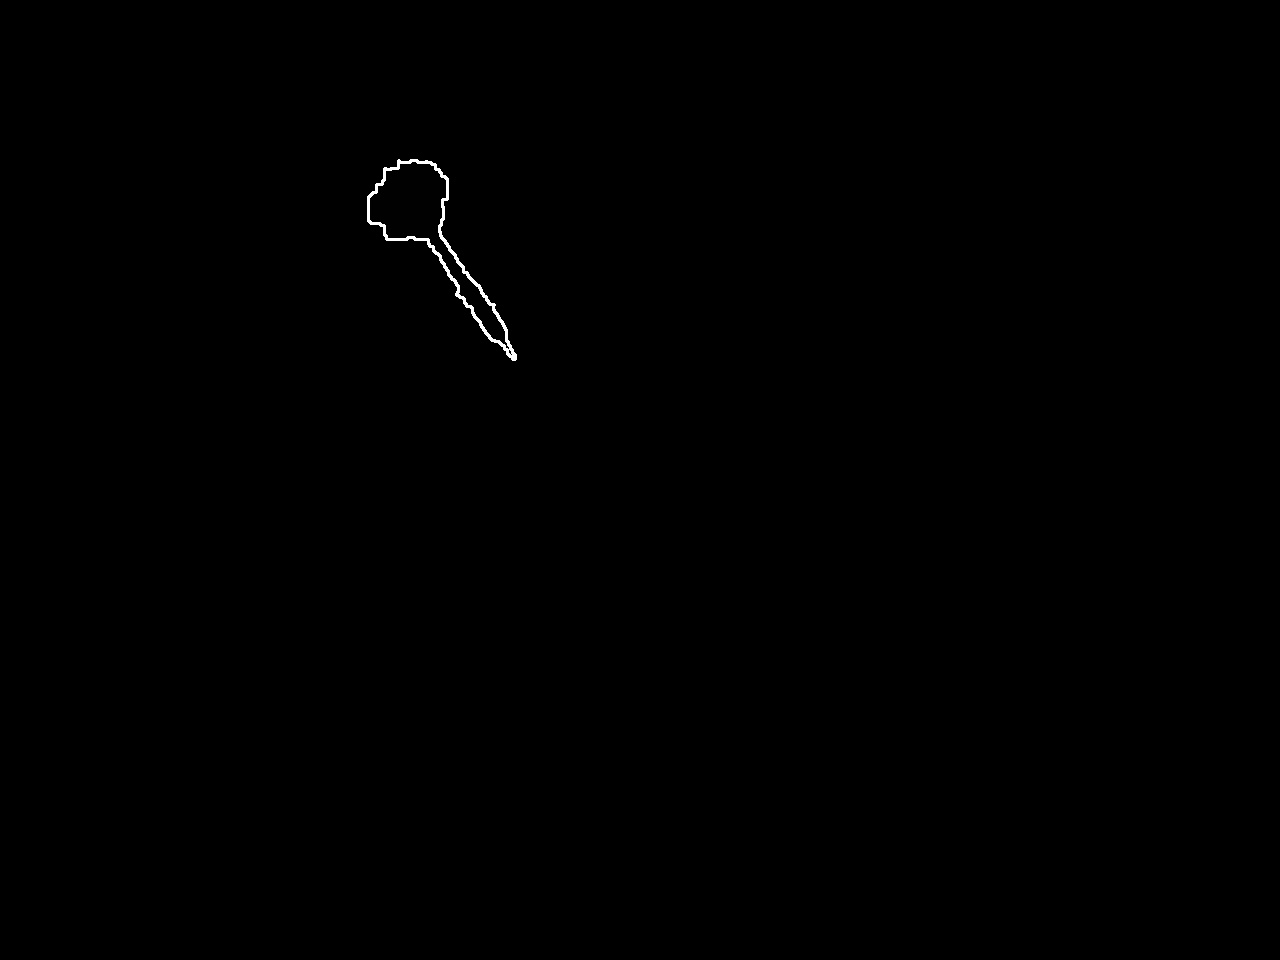
\includegraphics[scale=0.13]{./media/blobimgcontour.jpg}
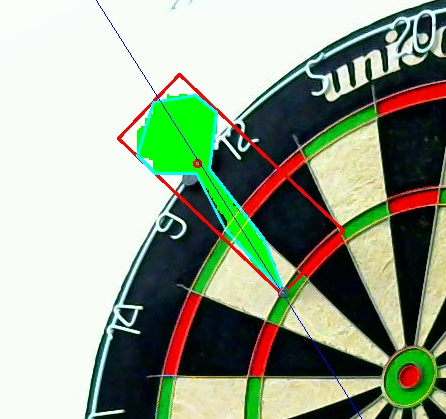
\includegraphics[scale=0.35]{./media/dartfeatures.jpg}

\end{overprint}
}

\frame{\frametitle{Dartspitzen Erkennung}
\begin{enumerate}
\item  Punkt der Kontur mit größter Distanz zum Schwerpunkt \pause 
\item  Schnittpunkt zwischen Gerade mit Bounding Rectangle \pause
\item  Punkt der approximierten Kontur mit größter Distanz zum Schwerpunkt \pause
\item  Schnittpunkt zwischen approximierten Kontur mit Bounding Rectangle \pause
\item  Schwerpunkt der restlichen Spitzen
\end{enumerate}
}

\frame{\frametitle{Dartspitzen Erkennung}
\begin{overprint}
\centering
\centerline{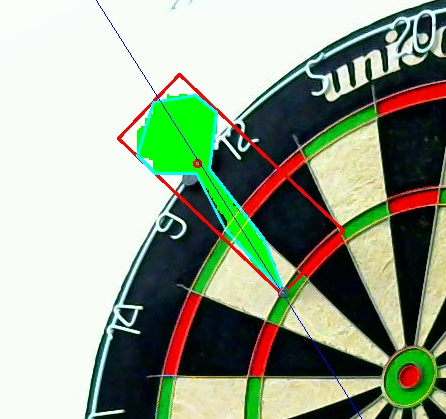
\includegraphics[scale=0.4]{./media/dartfeatures.jpg}}

\end{overprint}
}

\frame{\frametitle{Feldbestimmung}
\begin{enumerate}
\item  Alle fünf errechneten Bildpunkte verarbeitet \pause
\item  Mit Hilfe der Rotations- und Translationsmatrix \pause
\item  Objektpunkt auf Dartboardmodell anwenden
\end{enumerate}
}


\frame{\frametitle{Punkte Anzeige}
\begin{overprint}
\centering
\centerline{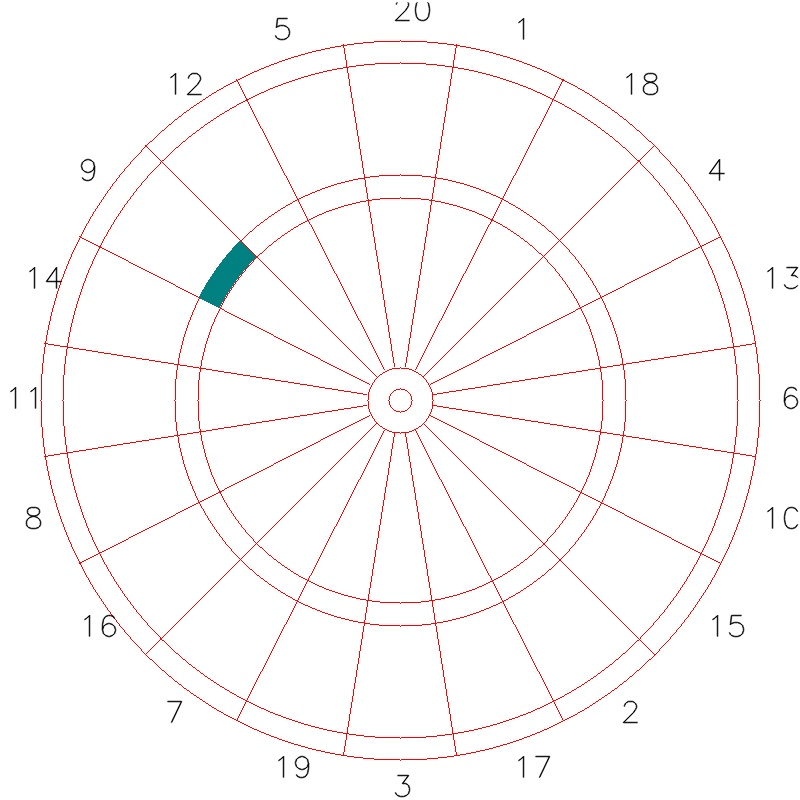
\includegraphics[scale=0.2]{./media/pointimg.jpg}}

\end{overprint}
}

\section{Evaluation} 
\subsection{Durchführung}
\frame{\frametitle{Testumgebung}
\begin{itemize}
\item  CPU i7 mit 4 Kernen je 4 Ghz und nVidia GTX 970\pause 
\item  Ubuntu 16.04 LTS \pause
\item  Python 3.0 und OpenCV 3.0 \pause
\item  Logitech C310 mit 1280x780 \pause
\item  Turnierscheibe \pause
\item  Kamera von unten auf Dartboard gerichtet 
\end{itemize}
}

\frame{\frametitle{Testumgebung}
\begin{overprint}
\centering
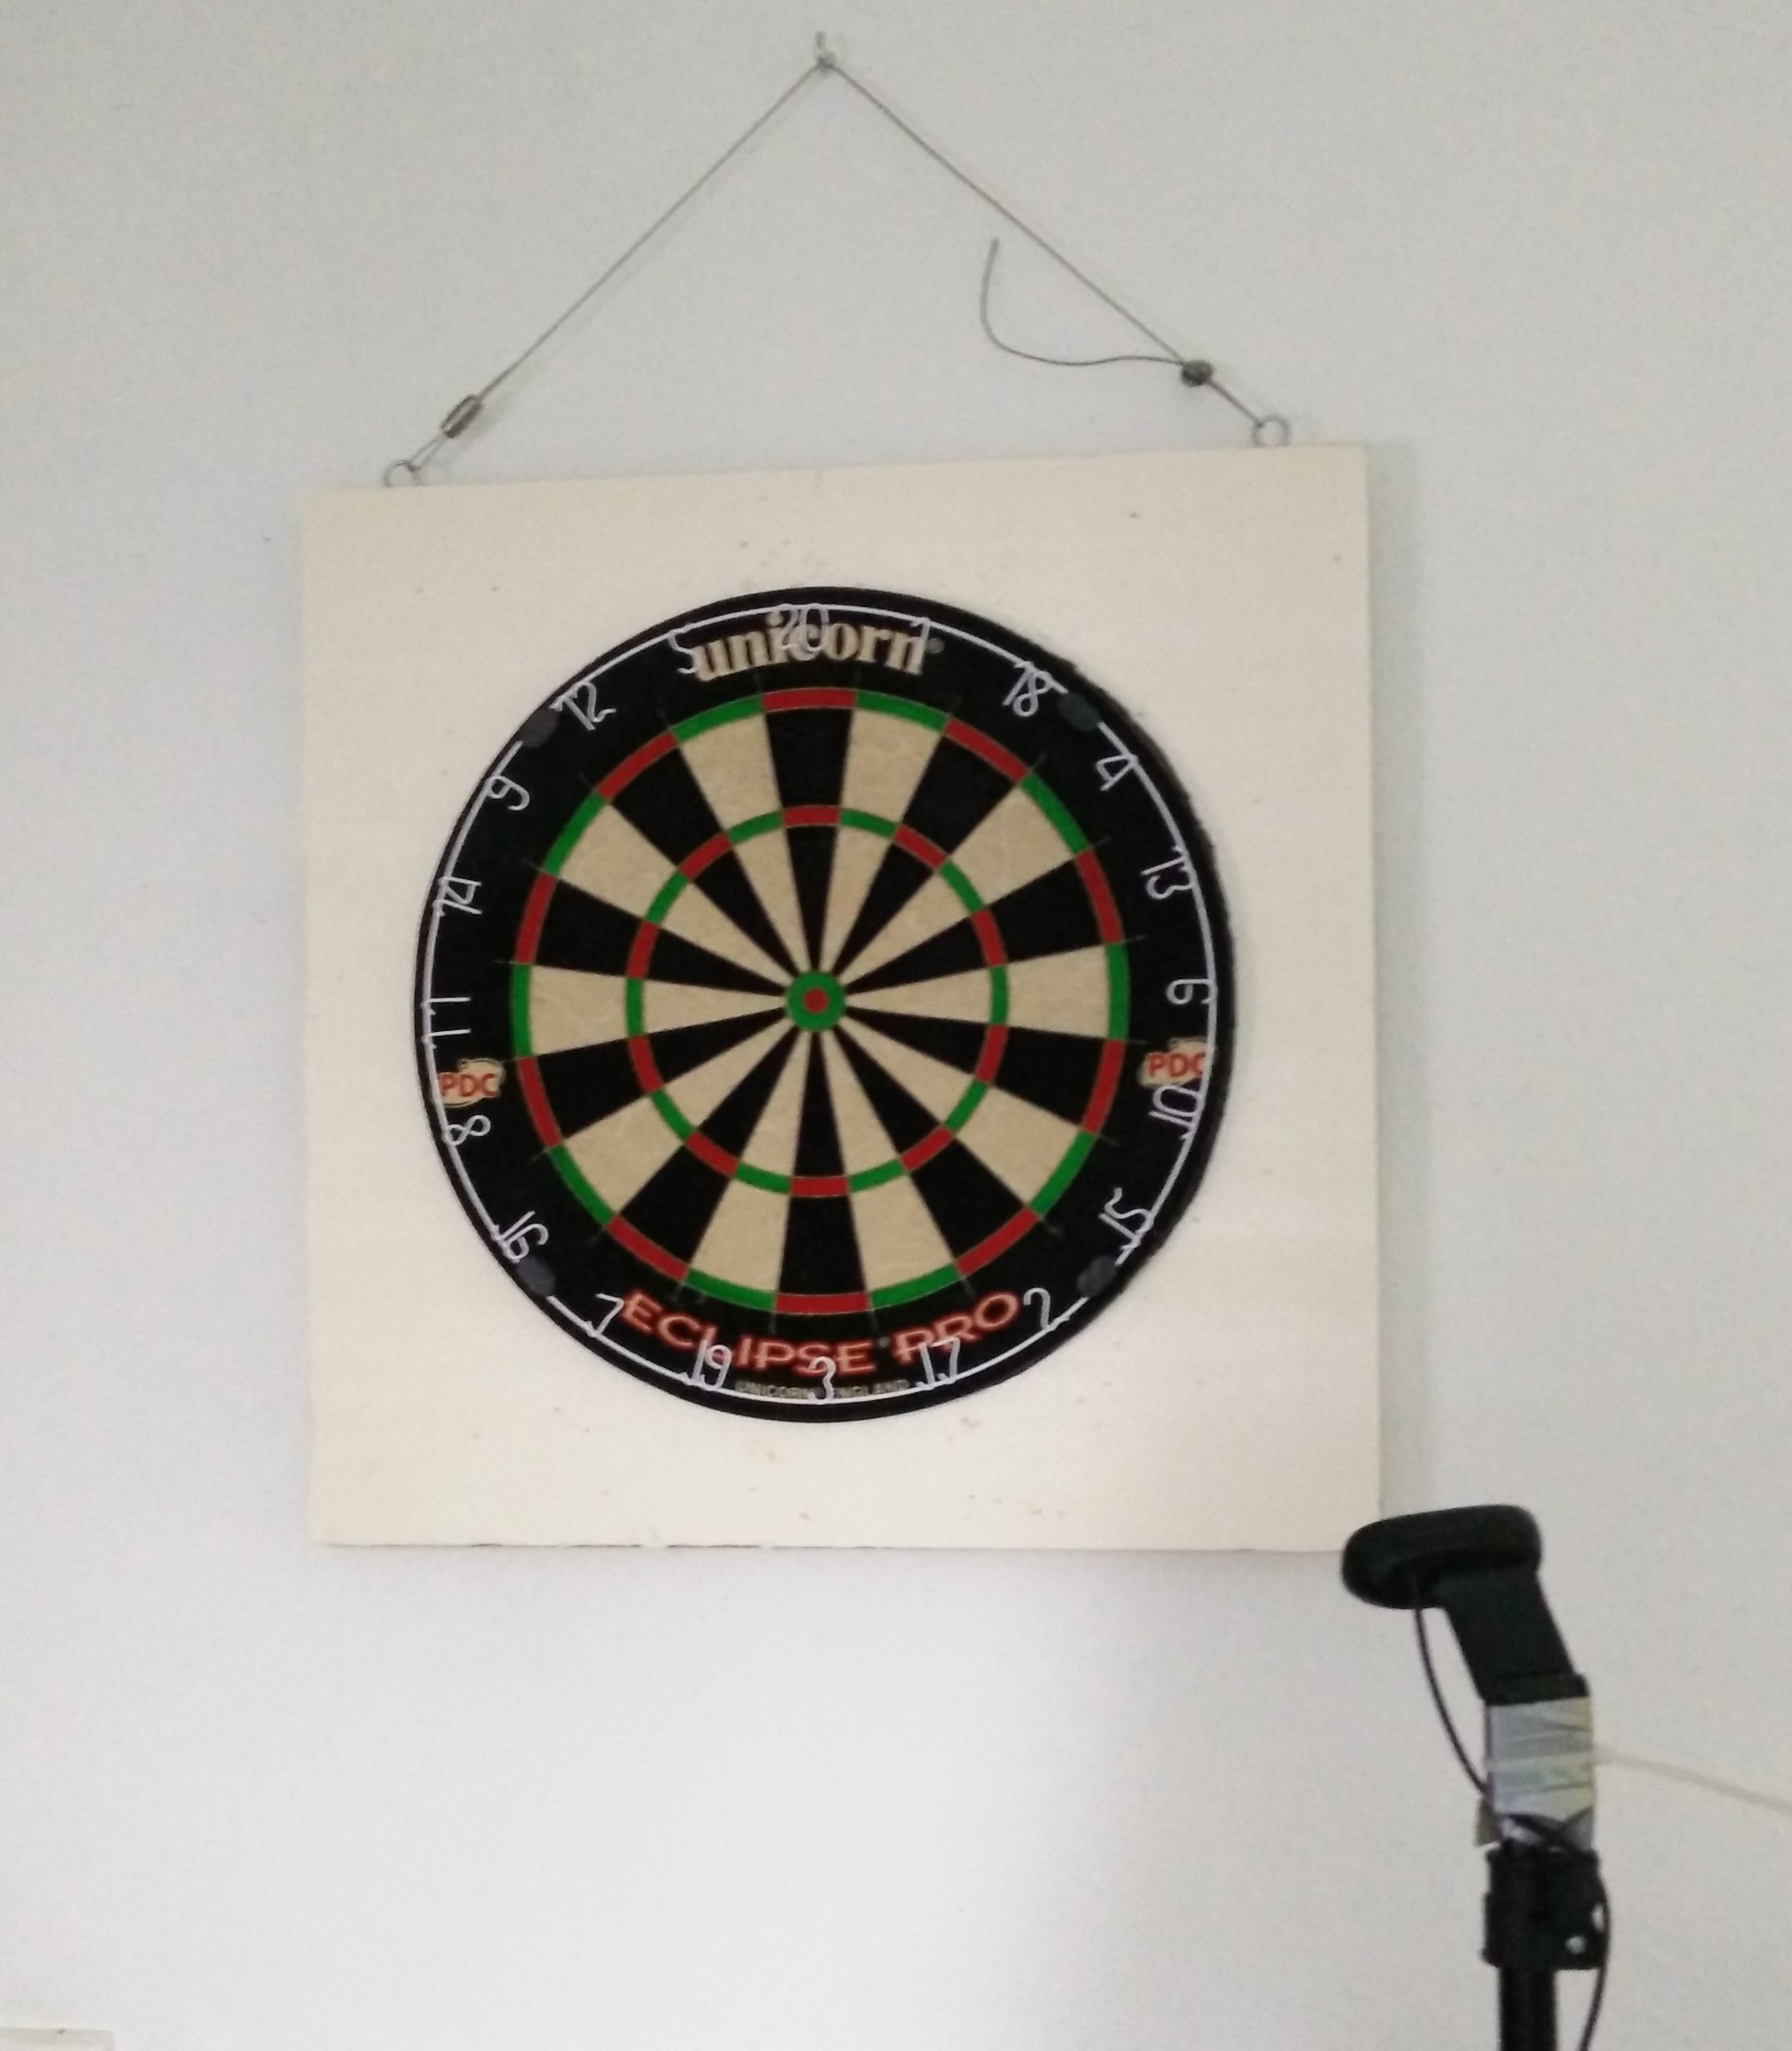
\includegraphics[scale=0.05]{./media/testsetup.jpg}
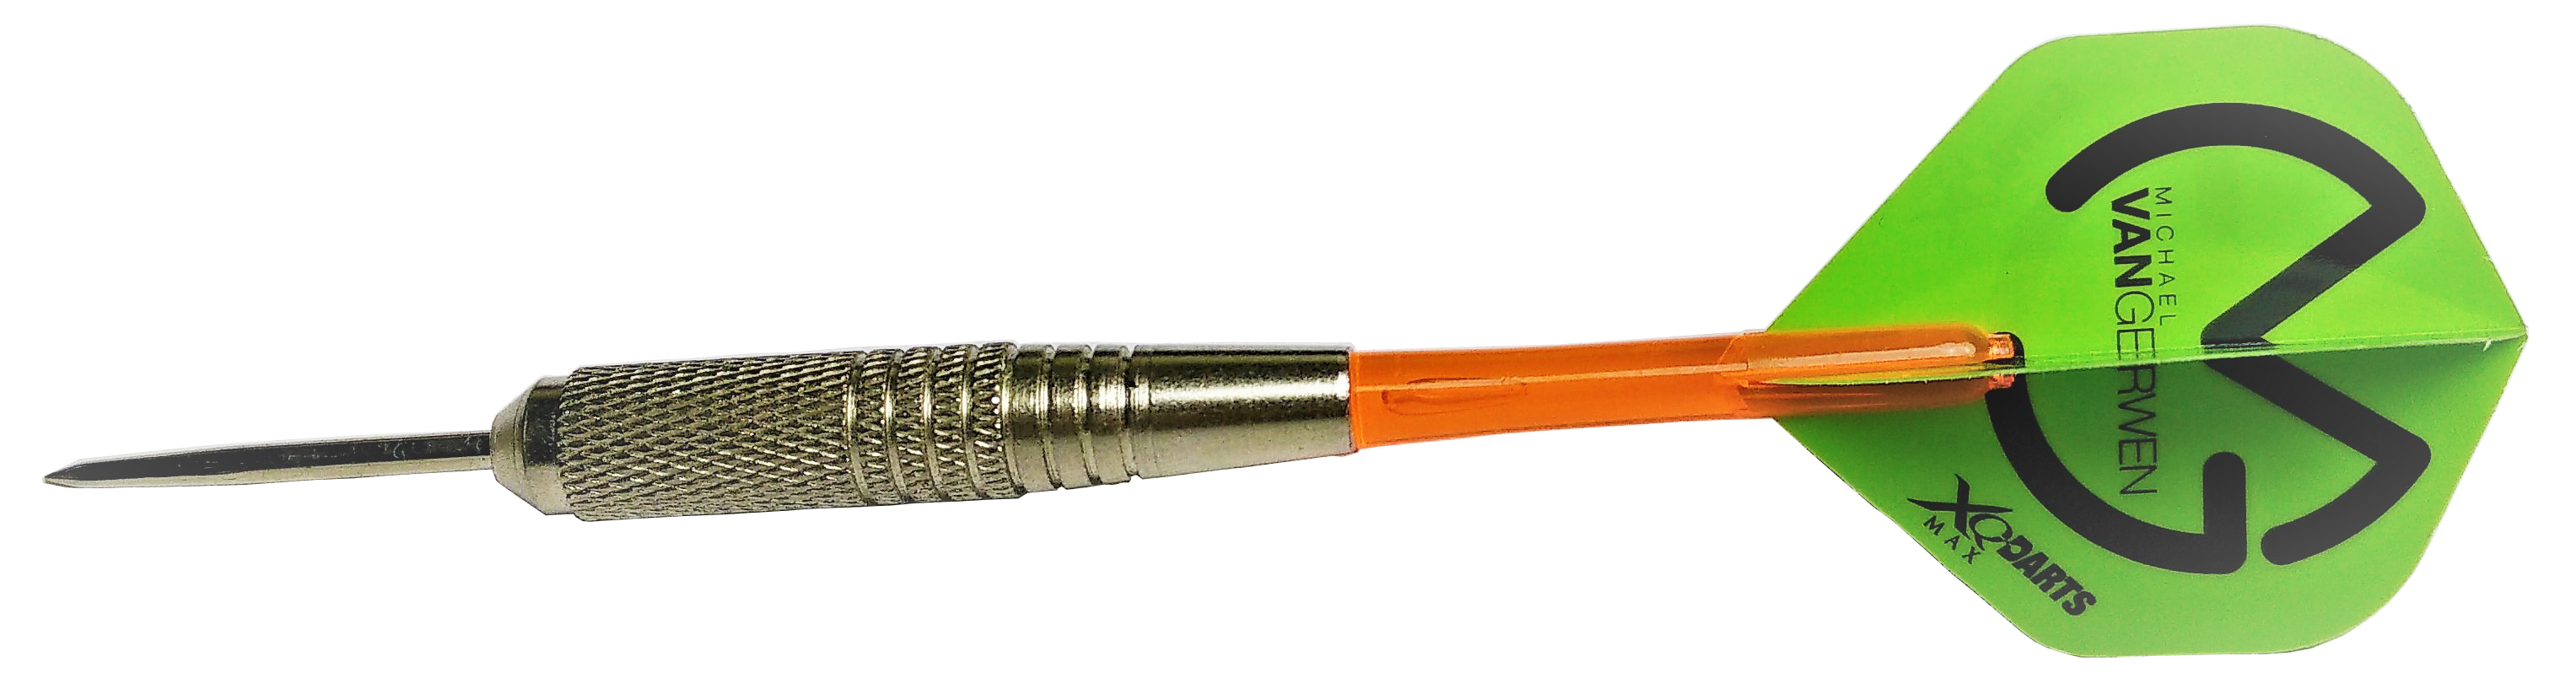
\includegraphics[scale=0.06]{./media/MyDart.png}

\end{overprint}
}

\frame{\frametitle{Testdaten}
\begin{itemize}
\item  Spielmodus "`Rennen"' \pause
\item  Rund 1000 Testwürfe durchgeführt \pause
\item  Berechnetes Feld aufgezeichnet 
\item  Tatsächliches Feld aufgezeichnet
\item  Verdeckung aufgezeichnet
\end{itemize}
}

\subsection{Resultate}
\frame{\frametitle{Alle Daten}
\begin{overprint}
\centering
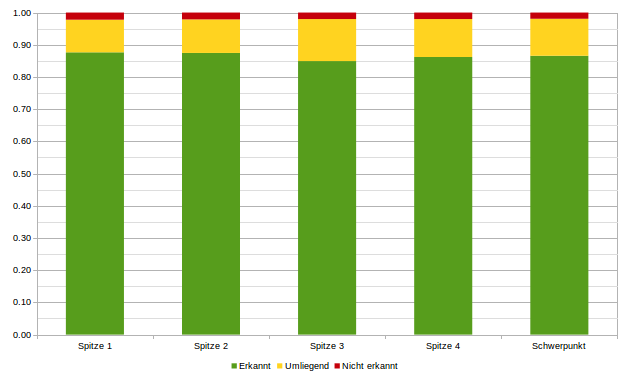
\includegraphics[scale=0.4]{./media/chartplain.png}

\end{overprint}
}

\frame{\frametitle{Verdeckung}
\begin{overprint}
\centering
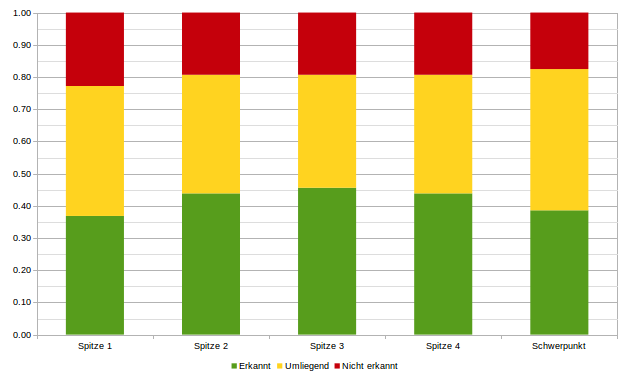
\includegraphics[scale=0.4]{./media/chartonlycovert.png}

\end{overprint}
}

\frame{\frametitle{Bereinigt}
\begin{overprint}
\centering
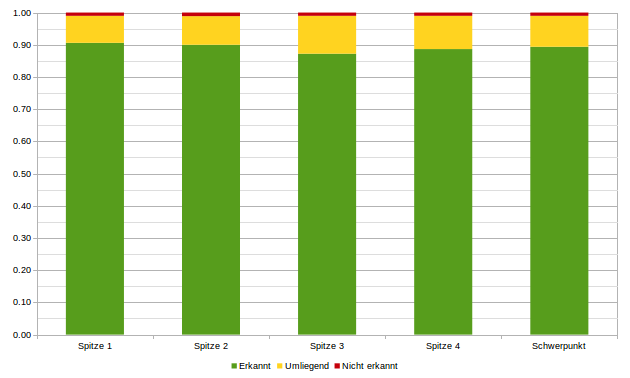
\includegraphics[scale=0.4]{./media/chartwithoutcovert.png}

\end{overprint}
}

\section{Ausblick und Fazit}
\frame{\frametitle{Mögliche Optimierungen}
\begin{itemize}
\item  Verbesserte Kamera verwenden \pause
\item  Zweite Kamera im anderen Winkel \pause
\item  Zweite Kamera für Stereosicht \pause
\item  3D Kamera verwenden \pause
\item  Verdeckung Softwareseitig erkennen
\end{itemize}
}

\frame{\frametitle{Fazit}
\begin{itemize}
\item  Einzelne Darts können erkannt werden \pause
\item Verdeckung verursacht Probleme \pause
\item Grundlage für die Erkennung wurde geschaffen
\end{itemize}
}



\end{document}
